\chapter{Resultados}
\label{ch:results}

%\begin{chapterquote}{Leslie Lamport}
%	Formal mathematics is nature's way of letting you know how sloppy
%your mathematics is.
%\end{chapterquote}

\noindent Los coeficientes $\beta_t$ que resultan de estimar la ecuación \ref{eq:1}, así como sus intervalos de confianza al 95\% con errores estándar cluster , se muestran en la Gráfica \ref{fig:1}. Las Gráficas \ref{fig:2} y \ref{fig:3} muestran los resultados de la misma regresión, pero restringida a las submuestras de salarios bajos y altos respectivamente. Los coeficientes $\beta_t$ que resultan de estimar la ecuación \ref{eq:2}, así como sus intervalos de confianza al 95\% con errores estándar cluster, se muestran en la Gráfica \ref{fig:4}. Las Gráficas \ref{fig:5} y \ref{fig:6} muestran los resultados de la misma regresión, pero restringida a las submuestras de salarios bajos y altos respectivamente.

En la primera parte de mi análisis, observo que el efecto del incremento al salario mínimo en la ZLFN sobre el empleo fue pequeño o inexistente. Esto se ilustra en la Gráfica \ref{fig:1} de resultados, donde se aprecia que los coeficientes de diferencias en diferencias para todos los años son cercanos a cero. Además, este comportamiento se mantiene después del aumento del salario mínimo en la ZLFN. Casi todos los intervalos de confianza de los coeficientes \textit{diff-in-diff} contienen al cero, salvo el correspondiente al segundo trimestre de 2019. La inclusión del cero en el intervalo de confianza indica en que el impacto del aumento al salario mínimo en la ZLFN sobre el empleo no fue estadísticamente significativo.      

\begin{figure}[H]
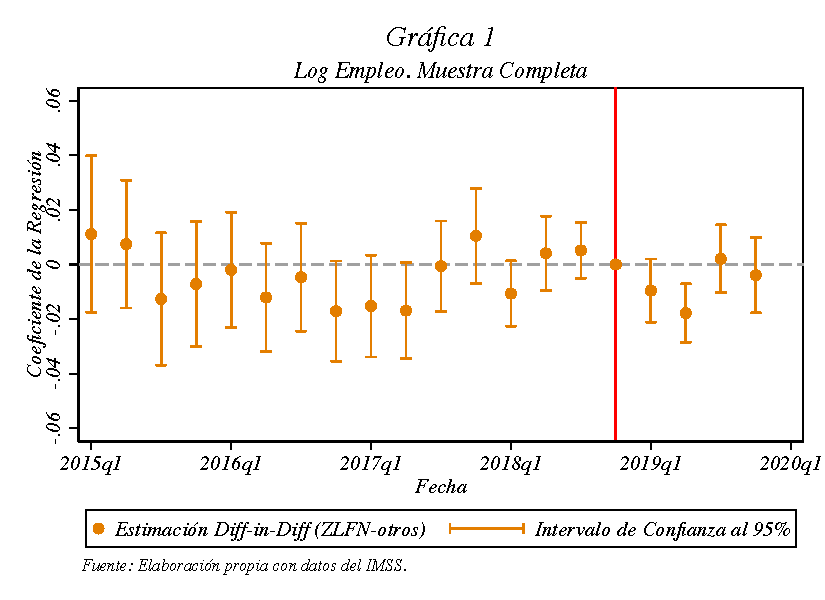
\includegraphics[width=0.9\textwidth]{Figures/LogEmpleo_MuestraCompleta.pdf}
\caption{Impacto del aumento en el salario en el empleo. Muestra completa.}
\label{fig:1}
\end{figure}


Es posible que la falta de un impacto significativo se deba a que el aumento al salario mínimo solamente afecta al empleo en la cola izquierda de la distribución de salarios, que contribuyen poco al empleo agregado. Sin embargo, al separar a los trabajadores por nivel salarial se aprecia que esto no es el caso. Si nos enfocamos únicamente en la submuestra de empleos bajos, es decir, gente que gana menos de dos salarios mínimos, vemos que todos los intervalos de confianza de los coeficientes \textit{diff-in-diff} contienen al cero. Efectivamente, si hacemos el mismo ejercicio para la submuestra de empleos altos, vemos que la anomalía vista en la muestra completa durante el segundo trimestre de 2019 se suscita por trabajadores pertenecientes a esta submuestra. Al observarla segunda gráfica se observa que, para la población de menores ingresos, un incremento al salario mínimo no tiene impactos sobre el empleo. Para la población en su totalidad, también es posible decir que el efecto del incremento al salario mínimo en la ZLFN es pequeño o nulo.

\begin{figure}[H]
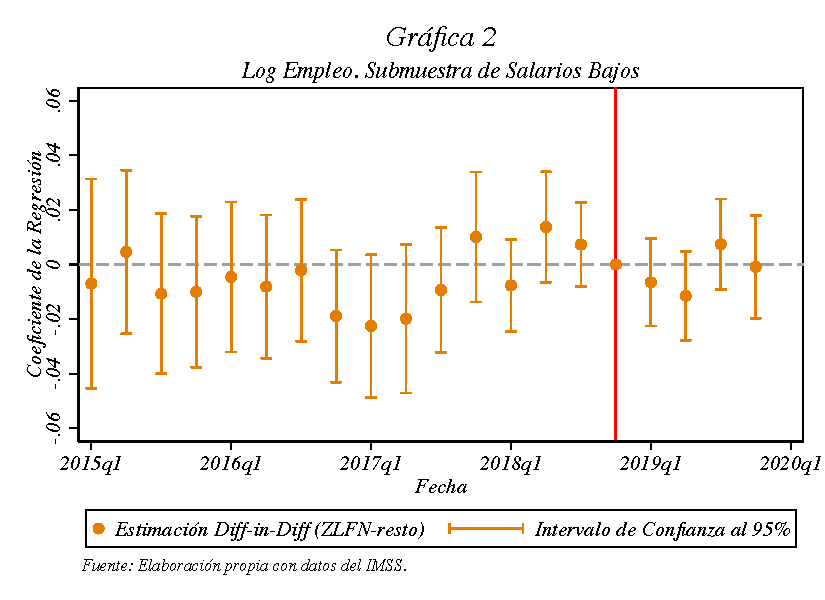
\includegraphics[width=\textwidth]{Figures/LogEmpleo_SalariosBajos.pdf}
\caption{Efecto del aumento del salario mínimo en el empleo. Submuestra salarios bajos.}
\label{fig:2}
\end{figure}

\begin{figure}[H]

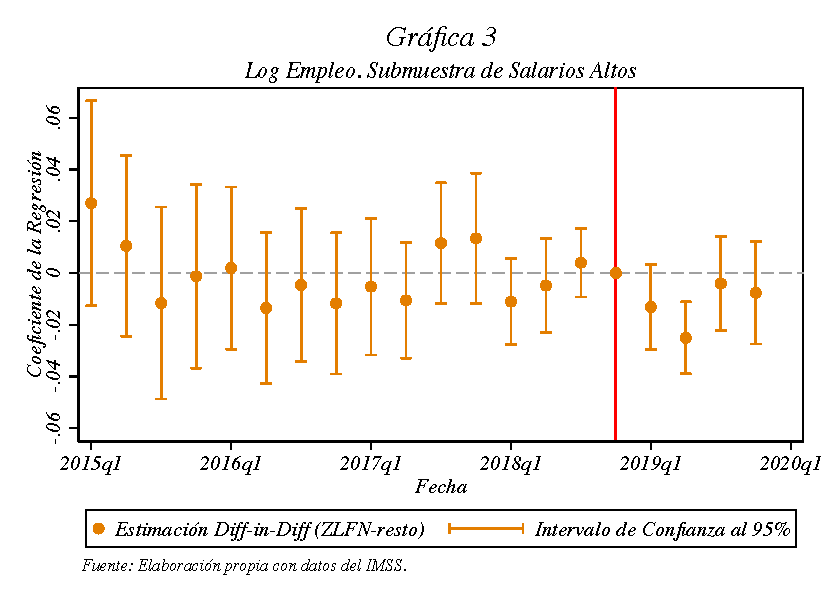
\includegraphics[width=\textwidth]{Figures/LogEmpleo_SalariosAltos.pdf}
\caption{Efecto del aumento del salario mínimo en el empleo. Submuestra salarios altos.}
\label{fig:3}
\end{figure}

Sin embargo, sí hay un impacto significativo sobre los salarios para todos los trabajadores, sobre todo dentro de la población de menores salarios. Al separar nuevamente a los trabajadores por nivel de salario, se observa que el aumento salarial causado por subir el salario mínimo es mucho mayor para niveles bajos de salarios que para niveles altos de salarios.

Los coeficientes que resultan de mi estrategia de diferencias en diferencias son estadísticamente significativos y positivos. Es decir, los salarios de cotización ante el IMSS de la ZLFN aumentan en mayor medida (aproximadamente 10\%) que el resto del país, producto del aumento diferenciado al salario mínimo en 2019. Además, al separar a los trabajadores por nivel salarial, encuentro que el efecto es mayor  para los trabajadores con menores salarios. Una explicación es que existe complementariedad entre ambos tipos de trabajos, otra que los salarios bajos se usan de referencia al negociar los salarios altos (el llamado efecto faro).

\begin{figure}[H]
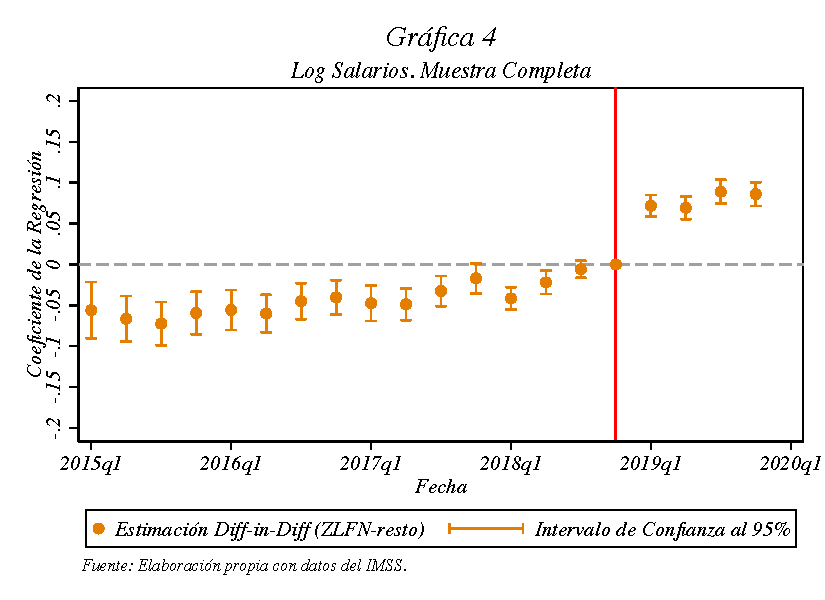
\includegraphics[width=\textwidth]{Figures/_LogSalarios_MuestraCompleta.pdf}
\caption{Efecto del aumento del salario mínimo en los salarios. Muestra completa.}
\label{fig:4}
\end{figure}

\begin{figure}[H]
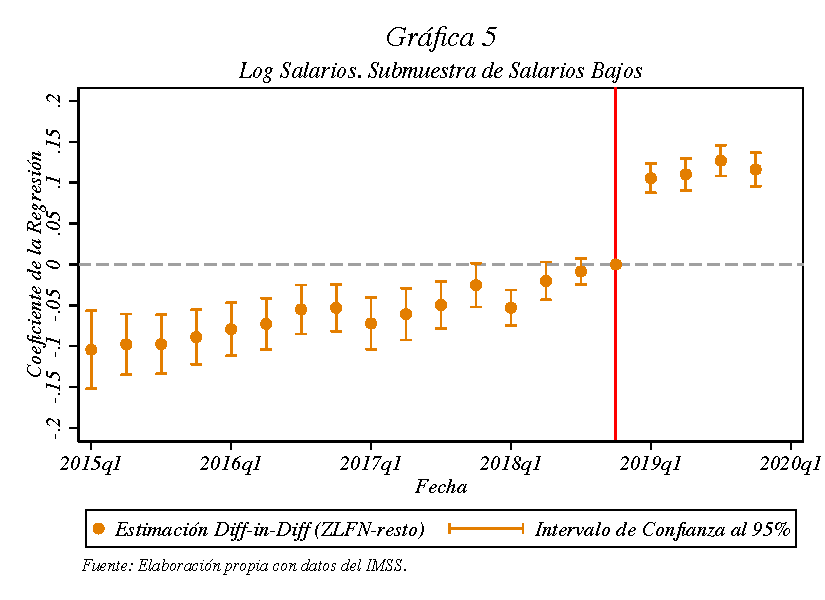
\includegraphics[width=\textwidth]{Figures/_LogSalarios_SalariosBajos.pdf}\caption{Efecto del aumento del salario mínimo en los salarios. Subuestra salarios bajos.}
\label{fig:5}
\end{figure}

\begin{figure}[H]
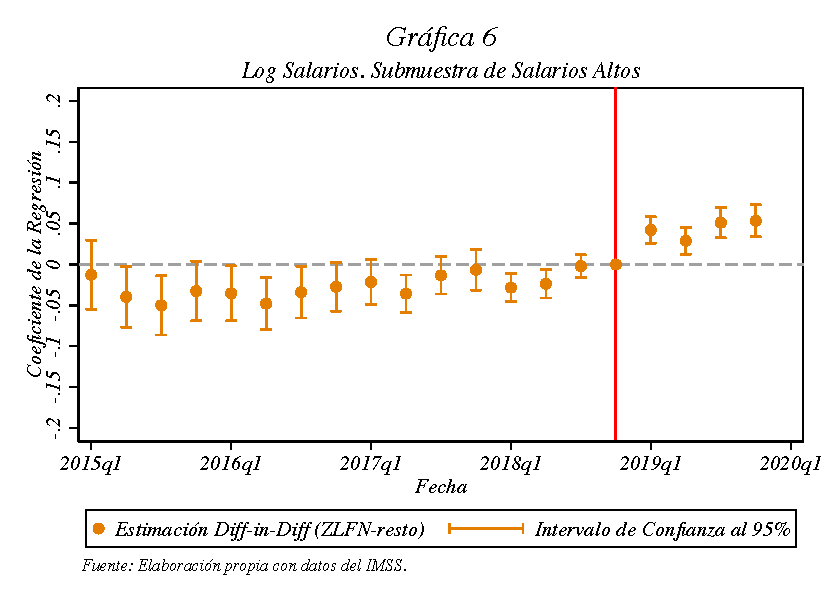
\includegraphics[width=\textwidth]{Figures/_LogSalarios_SalariosAltos.pdf}\caption{Efecto del aumento del salario mínimo en los salarios. Submuestra salarios altos.}
\label{fig:6}
\end{figure}

En resumidas cuentas, con respecto a la primera parte de mis estimaciones, subir el salario mínimo sí aumenta el salario de cotización de los trabajadores, sobre todo aquellos de bajos salarios, sin tener impacto significativo sobre el nivel de empleo. 

Si bien los coeficientes de la gráfica \ref{fig:4} antes de aumentar el salario mínimo muestran una suave tendencia creciente, el mayor cambio de un periodo a otro no excede 0.03. mientras,el cmabio después de aumentar el salario mínimo es de casi 0.1. Una historia similar puede contarse sobre las tendencias pre aumento del salario mínimo de \ref{fig:5} y \ref{fig:6}.

Para la segunda parte, resumo en tablas los coeficientes de las regresiones estimadas para ambas variables dependientes, cambiando solamente la medida de intensidad estatal. Los resultados de las regresiones \ref{eq:3} y \ref{eq:4} se muestran en las Tablas \ref{tab:2} y \ref{tab:3}, respectivamente.


Los datos expuestos en las Tablas \ref{tab:2} y \ref{tab:3} están redondeadas a tres cifras significativas. Observando la Tabla \ref{tab:2} se observa que, sin importar la medida que se opte por usar, el efecto de subir el salario mínimo es positivo , pero no estadísticamente significativo sobre el número de créditos. Es posible apreciar que, para la hipótesis nula de que los coeficientes son cero, el p-value para $\beta$ es alto sin importar cuál medida de intensidad estatal se utilice, por lo cual los coeficientes no son estadísticamente significativos. 

Aquí he estimado el coeficiente  que pondera al tratamiento, es decir el periodo a partir del cual se hace el aumento al salario mínimoy a la medida de intensidad estatal. Recordemos que esta medida es un proxy de qué tanto se ve afectada cada entidad federativa por la medida. Los resultados de las regresiones indican que el aumento al salario mínimo no trajo consigo un efecto significativo sobre el número de créditos otorgado por el INFONAVIT a trabajadores. Este primer resultado no es sorprendente, dado que el acceso a créditos INFONAVIT depende principalmente de contar con un salario formal y el aumento al salario mínimo no parece haber impactado de forma importante al total de empleos.

\begin{table}[H]
\caption{Impacto del aumento al salario mínimo en la ZLFN sobre el número de créditos INFONAVIT otorgados}
\label{tab:2}
\begin{adjustbox}{max width=\textwidth}
\begin{tabular}{lcccc}

\hline \\
 & & Logaritmo & de créditos & INFONAVIT  \\
 &  &  &  &  \\
Medidas de intensidad estatal & (1) & (2) & (3) & (4)  \\ \hline
 &  &  &  &  \\
\% de trabajadores que ganan entre 1 y 2 salarios mínimos que viven en la ZLFN & 0.00656 &  &  &  \\
 & (0.0852) &  &  &  \\
\% del total de empleos de trabajadores que ganan entre 1 y 2 salarios mínimos que viven en la ZLFN &  & 0.00902 &  &  \\
 &  & (0.285) &  &  \\
\% de trabajadores que ganan menos de 2 salarios mínimos que viven en la ZLFN &  &  & 0.00915 &  \\
 &  &  & (0.286) &  \\
\% del total de empleos de trabajadores que ganan menos de 2 salarios mínimos que viven en la ZLFN  &  &  &  & 0.00660 \\
 &  &  &  & (0.0852) \\
Constante & 7.959*** & 7.960*** & 7.960*** & 7.959*** \\
 & (0.0315) & (0.0315) & (0.0315) & (0.0315) \\
 &  &  &  &  \\
 Effectos fijos por estado  &  Sí &  Sí &  Sí & Sí \\
  Effectos fijos por periodo  &  Sí &  Sí &  Sí & Sí \\
Observaciones & 496 & 496 & 496 & 496 \\
 R-cuadrada & 0.975 & 0.975 & 0.975 & 0.975 \\ \hline
\multicolumn{5}{c}{ Errores estándar robustos y clusterizados por estado en paréntesis} \\
\multicolumn{5}{c}{ *** p$<$0.01, ** p$<$0.05, * p$<$0.1} \\
\multicolumn{5}{c}{Fuente: Elaboración propia con datos del IMSS e INFONAVIT.} \\

\end{tabular}
\end{adjustbox}

\end{table}


En contraste, de acuerdo con la Tabla \ref{tab:3}, para todas las medidas de intensidad estatal, el incremento al salario mínimo está asociado con un aumento en el monto de los créditos. En este caso, los coeficientes  son positivos  y estadísticamente significativos, como indican los p-values menores a 5\%. A continuación, se muestran los coeficientes  para diferentes medidas de intensidad estatal. Para darnos idea del tamaño de la política diferenciada en la ZLFN, en particular para el coeficiente correspondiente a la segunda medida de intensidad la subida del salario mínimo causó que si un estado tenía un punto porcentual más de trabajadores que ganan entre uno y dos salario mínimos entonces los trabajadores de ese estado recibieron 65 millones de pesos adicionales de hipoteca por parte del INFONAVIT.

La combinación de ambos resultados muestra que el INFONAVIT amplía el monto de los créditos sin cambiar el número de créditos que otorga. Esta conclusión es importante porque indica que efectivamente el aumento al salario mínimo permitió a los trabajadores de la ZLFN acceder a montos más altos de crédito hipotecario.



\begin{table}[H]
\caption{Impacto del aumento al salario mínimo en la ZLFN sobre el monto de créditos INFONAVIT}
\label{tab:3}
\begin{adjustbox}{max width=\textwidth}
\begin{tabular}{lcccc}
 &  &  &  &  \\
\hline
 & & Monto de & crédito & INFONAVIT  \\
 &  &  &  &  \\
Medidas de intensidad estatal & (1) & (2) & (3) & (4)  \\ \hline
 &  &  &  &  \\
\% de trabajadores que ganan entre 1 y 2 salarios mínimos que viven en la ZLFN & 0.191** &  &  &  \\
 & (0.0863) &  &  &  \\
 \% del total de empleos de trabajadores que ganan entre 1 y 2 salarios mínimos que viven en la ZLFN &  & 0.650** &  &  \\
 &  & (0.300) &  &  \\
\% de trabajadores que ganan menos de 2 salarios mínimos que viven en la ZLFN &  &  & 0.651** &  \\
 &  &  & (0.300) &  \\
\% del total de empleos de trabajadores que ganan menos de 2 salarios mínimos que viven en la ZLFN  &  &  &  & 0.191** \\
 &  &  &  & (0.0863) \\
Constante & 1.449*** & 1.450*** & 1.450*** & 1.449*** \\
 & (0.0315) & (0.0315) & (0.0315) & (0.0315) \\
 &  &  &  &  \\
 Effectos fijos por estado  &  Sí &  Sí &  Sí & Sí \\
  Effectos fijos por periodo  &  Sí &  Sí &  Sí & Sí \\
Observaciones & 496 & 496 & 496 & 496 \\
 R-cuadrada & 0.977 & 0.977 & 0.977 & 0.977 \\ \hline
\multicolumn{5}{c}{ Errores estándar robustos y clusterizados por estado en paréntesis} \\
\multicolumn{5}{c}{ *** p$<$0.01, ** p$<$0.05, * p$<$0.1} \\
\multicolumn{5}{c}{Fuente: Elaboración propia con datos del IMSS e INFONAVIT.} \\
\end{tabular}

\end{adjustbox}
\end{table}

Ante el aumento de la oferta de crédito esperaríamos que se ajustara o la oferta de vivienda o su precio. En caso de que la oferta fuera muy inelástica, todo el impacto debería trasladarse al precio y por tanto implicar que la calidad de la vivienda a la que tendrían acceso las personas que recibieron ese aumento no cambiaría. El impacto del aumento en el salario mínimo en los precios de vivienda no es significativo como se aprecia en la siguiente gráfica. Todos los intervalos de confianza al 95\% toman al cero. Este resultado sugiere que la oferta de vivienda para el sector de trabajadores que observaron un aumento en el monto de las hipotecas disponibles es relativamente elástica. Lo que implica que el aumento en el crédito disponible puede estarse traduciendo en el acceso a vivienda de mayor calidad. 

Cabe notar el comportamiento atípico de los intervalos de confianza. Dado que tengo la misma cantidad de datos para todas las fechas, la explicación de que aumente el error pudiera ser que tengo pocas unidades en las cuales aumenta el salario mínimo aumentó frente a muchos municipios en los que no. En ese sentido, es necesario un análisis adicional de los precios de vivienda para asegurar que en efecto no cambiaron. Presento el control sintético correspondiente en la gráfica \ref{fig:10}.

\begin{figure}[H]
\includegraphics[width=\textwidth]{Figures/Precios_Muestracompleta.pdf}
\caption{Efecto del aumento en el salario mínimo en los precios de vivienda.}
\label{fig:7}
\end{figure}

Además, al analizar el mercado de crédito privado, resulta que el impacto del aumento del salario mínimo tampoco fue significativo. Sólo un par de intervalos están ligeramente alejados del cero después de la entrada en vigor de la ZLFN. Podemos conjeturar que los créditos INFONAVIT absorbieron todo el efecto del salario mínimo. Tiene sentido que sea así ya que el pago de hipoteca del INFONAVIT se hace a través de un descuento de nómina. A diferencia de un banco privado, donde se debe manifestar la intención de adquirir y pagar una hipoteca, es relativamente sencillo para el INFONAVIT cobrar su cartera.

\begin{figure}[H]
\includegraphics[width=\textwidth]{Figures/Creditos_Muestracompleta.pdf}
\caption{Efecto del aumento en el salario mínimo en el monto otorgado de crédito hipotecario privado.}
\label{fig:8}
\end{figure}

\begin{figure}[H]
\includegraphics[width=\textwidth]{Figures/Cantidad_Muestracompleta.pdf}
\caption{Efecto del aumento en el salario mínimo en la cantidad de créditos hipotecarios privados otorgados.}
\label{fig:9}
\end{figure}

Por último, presento las estimaciones del control sintético en precios de la vivienda. Al respecto, es importante considerar el posible sesgo por tener tan pocas unidades tratadas. Como se puede observar, el comportamiento del control sintético es prácticamente el mismo  que el de la variable observada después del aumento al salario mínimo. En ese sentido, se mantiene la conclusión del método de diferencias en diferencias: no hubo un cambio en precios derivado de la implementación del aumento al salario mínimo en la ZLFN.

\begin{figure}[H]
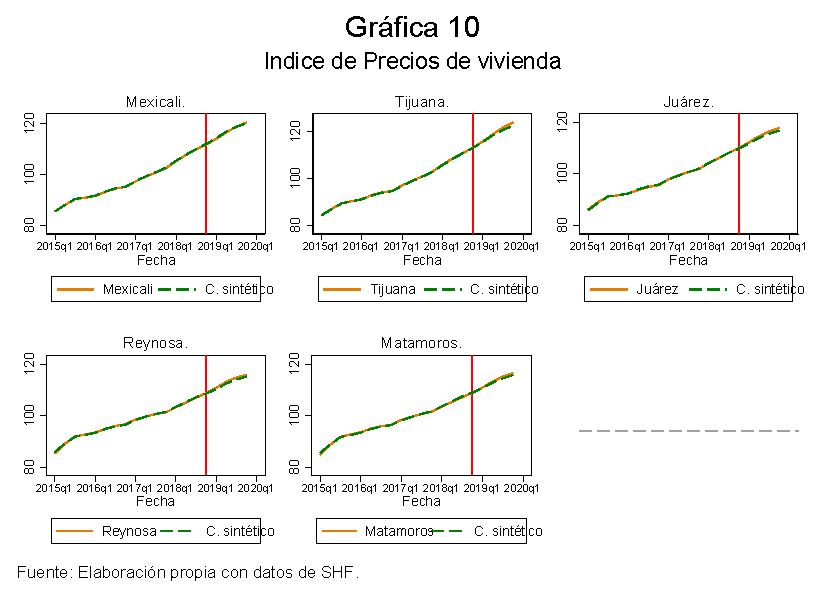
\includegraphics[width=\textwidth]{Figures/synth.pdf}
\caption{Control sintético para precios de vivienda.}
\label{fig:10}
\end{figure}
